
\chapter{Analysis by Cover Type}
\label{ch:covtype}
We defined 31 distinct land cover types in the Yuba River watershed and surrounding area for the purposes of \textsc{RMLands} simulations (Table~\ref{covertable}). A few of these were located in the buffer, but not the project area. Several others were treated as \emph{static} in the simulation: they did not undergo vegetation transitions over time or in response to fire. However, four of the \emph{static} types were allowed to experience wildfires: Agriculture, Grassland, Meadow, and Urban. Grasslands may experience fire, but because they are expected to recover from fire in less than five years (the length of one timestep in our simulation), we assume they remain constant in composition and structure. The discussion that follows focuses on the nine cover types found within the core project area that were treated as dynamic in the model and that occurred over an extent of at least 1000 ha in the project area. For each of these cover types, we briefly describe the simulated disturbance regime (i.e., spatial extent and distribution, frequency and temporal variability) associated with each relevant disturbance process, the vegetation dynamics resulting from the interplay between these disturbance processes and succession, and an examination of the cover type’s current departure from the simulated HRV. 

%\subsection{Curl-leaf Mountain Mahogany}
%\subsection{Lodgepole Pine} 
%\subsection{Lodgepole Pine with Aspen}
%\subsection{Mixed Evergreen - Ultramafic} 
%\subsection{Montane Riparian} 
%\subsection{Oak Woodland} 
%\subsection{Red Fir - Ultramafic} 
%\subsection{Red Fir with Aspen} 
%\subsection{Sierran Mixed Conifer with Aspen} 
%\subsection{Subalpine Conifer} 
%\subsection{Western White Pine} 


%topics
% CHECK disturbed area
% climate? tpi? - Looked at climate for OCFW...basically the same as for landscape. not sure what it adds

%%%%%%%%%%%%%%%%%%%%%%%%%%%%%%%%%%%%%%%%%%%%%%%%%%%%%%%%%%%%%%%%%%%%%%%%%%%%%
%%%%%%%%%%%%%%%%%%%%%%%%%%%%%%%%%%%%%%%%%%%%%%%%%%%%%%%%%%%%%%%%%%%%%%%%%%%%%
%%%%%%%%%%%%%%%%%%%%%%%%%%%%%%%%%%%%%%%%%%%%%%%%%%%%%%%%%%%%%%%%%%%%%%%%%%%%%
%%%%%%%%%%%%%%%%%%%%%%%%%%%%%%%%%%%%%%%%%%%%%%%%%%%%%%%%%%%%%%%%%%%%%%%%%%%%%
%%%%%%%%%%%%%%%%%%%%%%%%%%%%%%%%%%%%%%%%%%%%%%%%%%%%%%%%%%%%%%%%%%%%%%%%%%%%%

%\clearpage
\section{Mixed Evergreen - Mesic} 

\begin{figure}[!htbp]
  \centering
  \subfloat[][]{
    \centering
    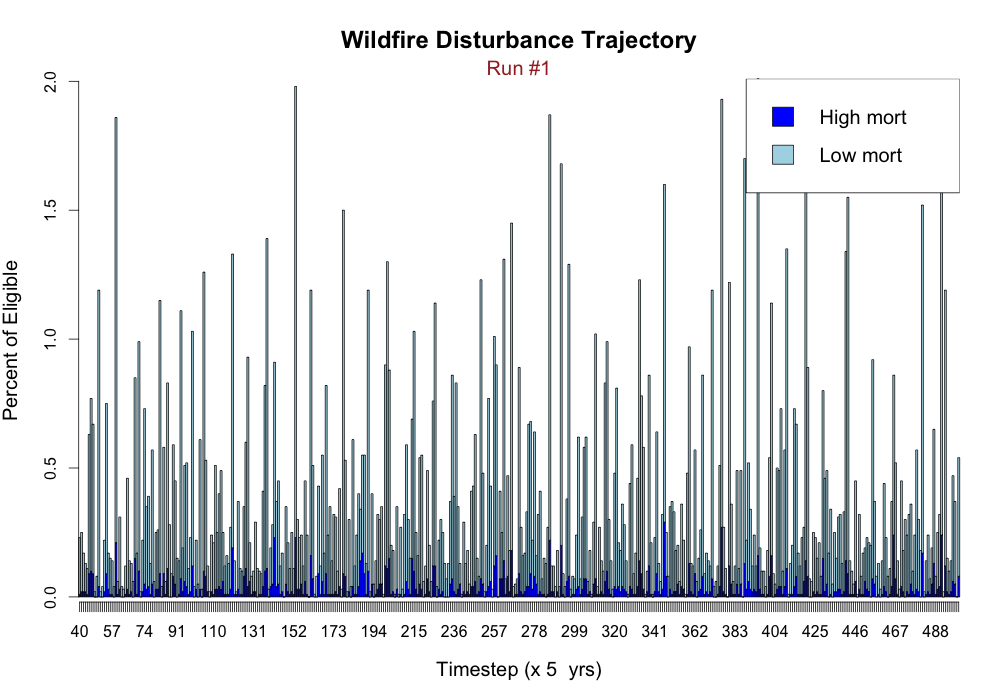
\includegraphics[width=0.5\textwidth]{/Users/mmallek/Tahoe/Report2/images/darea_megm.png}
    }%
  \subfloat[][]{
    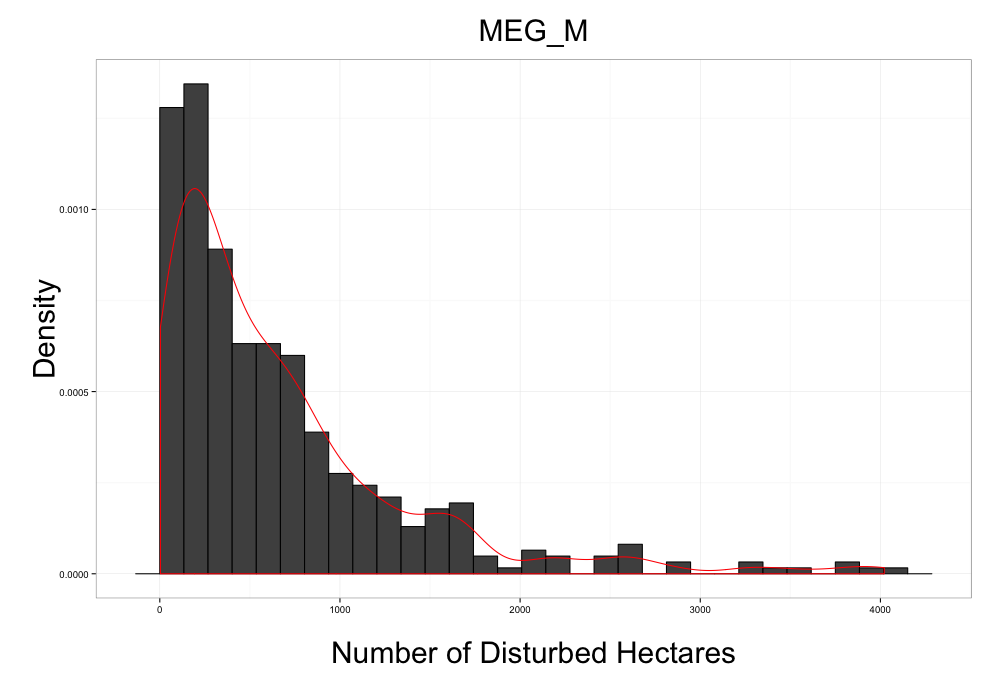
\includegraphics[width=0.5\textwidth]{/Users/mmallek/Tahoe/Report2/images/darea_hist_megm.png}
    }
  \caption{(a) \small Disturbance trajectory for Mixed Evergreen - Mesic. High mortality fire in dark blue; low mortality fire in light blue. (b) Histogram of disturbed hectares with density curve overlaid.} 
  \label{fig:darea_megm}
\end{figure}

Mixed Evergreen - Mesic (\textsc{meg\_m}) is a somewhat common cover type within the core project area, encompassing 7,273 ha and comprising roughly 4\% of the project area. The frequency and extent of simulated wildfires in mesic mixed evergreen forest varied markedly across the landscape (Figure~\ref{fig:darea_megm} and Table~\ref{tab:darea_megm}). %
%
While mesic mixed evergreen forests always experienced some wildfire during the simulation, during a typical five year period wildfires burned a small portion of the cover type, but the impacts were mostly low mortality. Low mortality fires were eight times as frequent as high mortality fires. Less than 1\% of the cover type (72 ha) burned during 9\% of the timesteps. Much more common were timesteps in which over 10\% of the landscape burned, which occurred about once in 17 years. The median proportion burned was 6\%. Seldom did large extents burn, at any mortality level, although roughly once every 68 years, more than 25\% of the cover type burned. We never observed a timestep during which more than 50\% of these forests experienced wildfire. The maximum extent burned within the cover type was about 48\% (about 3,500 ha). %
%
Under this wildfire regime, the grand mean return interval between fires (of any mortality level) varied widely from 19 years to more than 500 years, with a median of 62 years (Figure~\ref{fig:preturn_megm}). The median return interval and rotation values were influenced primarily by the dominant fire type, low mortality. Mesic mixed evergreen forests had a low mortality fire rotation of 63 years and a high mortality fire rotation of 534 years. %
%
In general, return intervals and canopy cover varied spatially across the forest and decreased with increasing TPI, reflecting our parameterization, which was based on the theory that higher, more southerly aspects are drier and more susceptible to fires. Canopy cover decreased by about 3\% when comparing minimum to maximum TPI (Table~\ref{tab:tpi_cc}). %
%
Finally, when stands of mesic mixed evergreen forests were adjacent to cover types with shorter return intervals, they also exhibited shorter return intervals, reflecting the importance of landscape context on fire regimes.

%%%
The age structure and dynamics of mesic mixed evergreen forest illustrates the interaction between disturbance and succession processes. We focus our analysis on the 5$^{\text{th}}$ to 95$^{\text{th}}$ percentile range of variability for our simulation (excluding the equilibration period). %
%
The distribution of area among stand conditions within mesic mixed evergreen forest fluctuated over time (Figure~\ref{fig:covcond_megm}). Because high mortality fire is very rare in this cover type, and the time to reaching a Late Development stage is relatively short (Appendix \ref{sec:covertypedesc}), the vast majority of the landscape, varying from 71\% to 88\%, was in the Late Development - Closed condition during the simulation (Table~\ref{tab:covcond1}). %
%
The seral-stage distribution appeared to be in dynamic equilibrium (i.e., the percentage in each stand condition varied about a stable mean). Our calculated current seral-stage distribution was never observed under the simulated HRV (Table~\ref{tab:covcond1}). The most notable departure was the shift from Mid Development to Late Development condition classes. About 52\% of the current landscape is comprised of the mesic mixed evergreen forest in mid development conditions, but the late development conditions were always dominant under the simulated HRV. The current proportions of all mid development canopy cover levels are higher than at any point during the HRV. As described above, much of the shift from the dominance of mid development conditions observed in the current distribution to the dominance by late development conditions during the HRV can be attributed to the prodigious increase in the extent of Late Development - Closed (from 29\% to 71-88\%), although Late Development - Moderate was also well represented, with an HRV from 6\%--15\%. The Early Development condition is also more common on the current landscape than during the simulation.

The spatial configuration of stand conditions fluctuated markedly over time as well, although there was considerable variation in the magnitude of variability among configuration metrics (Appendix \ref{sec:full-class-results}). Area-weighted patch and core area, edge density, and patch density exhibited the greatest variability over time. Because the landscape is so dominated by the Late Development - Closed and Moderate conditions, we focus on the configuration metrics for these classes. In general, the current landscape contains fewer, smaller, and more clumped patches than existed under the simulated HRV. Current patches in Late Development - Closed are less geometrically complex and have less area in cores than during the simulated HRV.


\begin{table}[!htbp]
\centering
\caption{\small Disturbed area summary statistics for Mixed Evergreen - Mesic. Proportions shown are relative to the total area of Mixed Evergreen - Mesic.}
\label{tab:darea_megm}
	\begin{tabular}{@{}llll@{}} 
	\toprule
	\textbf{\begin{tabular}[c]{@{}l@{}}Summary Statistic \\ (disturbed area/timestep)\end{tabular}} & \textbf{\begin{tabular}[c]{@{}l@{}}Low  Mortality\end{tabular}} & \textbf{\begin{tabular}[c]{@{}l@{}}High  Mortality\end{tabular}} & \textbf{\begin{tabular}[c]{@{}l@{}}Any  Mortality\end{tabular}} \\ \midrule
	Minimum       & 0.06       &  0.00       & 0.06       \\
	Maximum       & 44.44       & 6.90       & 48.25        \\
	Median        & 4.90       &  0.49       & 5.66       \\
	Mean          & 7.91       &  0.94       & 8.84       \\ 
	\textbf{Fire Rotation}  &  63  &  534  &  57  \\ \bottomrule
	\end{tabular}
\end{table}

%%%%%%%%%%%%%%%%%%%%%%%%%%%%%%%%%%%%%%%%%%%%%%%%%%%%%%%%%%%%%%%%%%%%%%%%%%%%%
%%%%%%%%%%%%%%%%%%%%%%%%%%%%%%%%%%%%%%%%%%%%%%%%%%%%%%%%%%%%%%%%%%%%%%%%%%%%%
%%%%%%%%%%%%%%%%%%%%%%%%%%%%%%%%%%%%%%%%%%%%%%%%%%%%%%%%%%%%%%%%%%%%%%%%%%%%%
%%%%%%%%%%%%%%%%%%%%%%%%%%%%%%%%%%%%%%%%%%%%%%%%%%%%%%%%%%%%%%%%%%%%%%%%%%%%%
%%%%%%%%%%%%%%%%%%%%%%%%%%%%%%%%%%%%%%%%%%%%%%%%%%%%%%%%%%%%%%%%%%%%%%%%%%%%%

%\clearpage
\section{Mixed Evergreen - Xeric} 

\begin{figure}[!htbp]
  \centering
  \subfloat[][]{
    \centering
    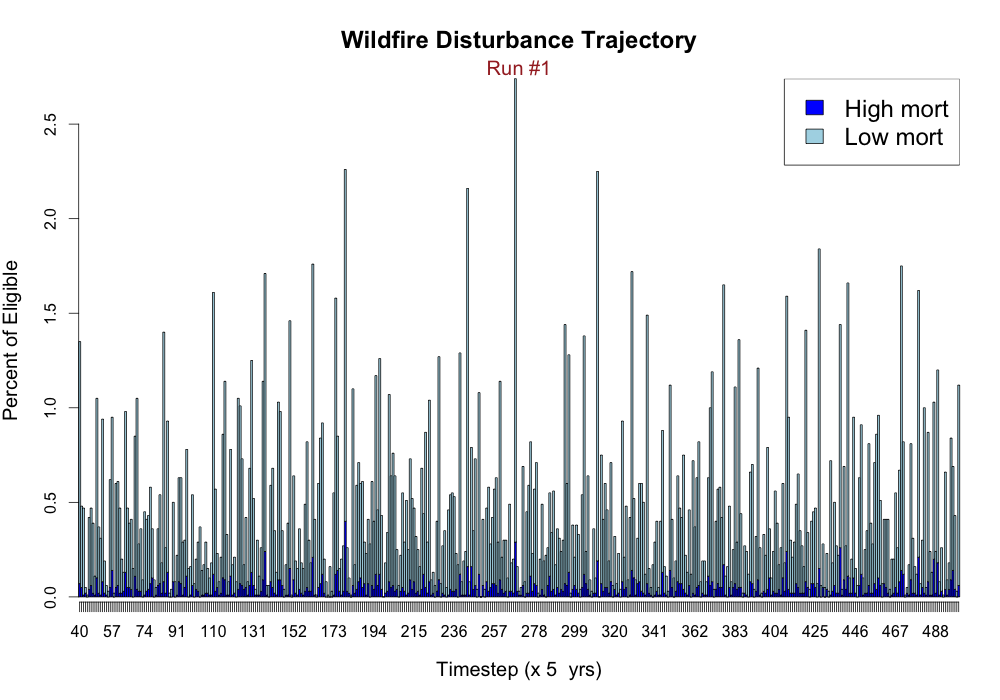
\includegraphics[width=0.5\textwidth]{/Users/mmallek/Tahoe/Report2/images/darea_megx.png}
    }%
  \subfloat[][]{
    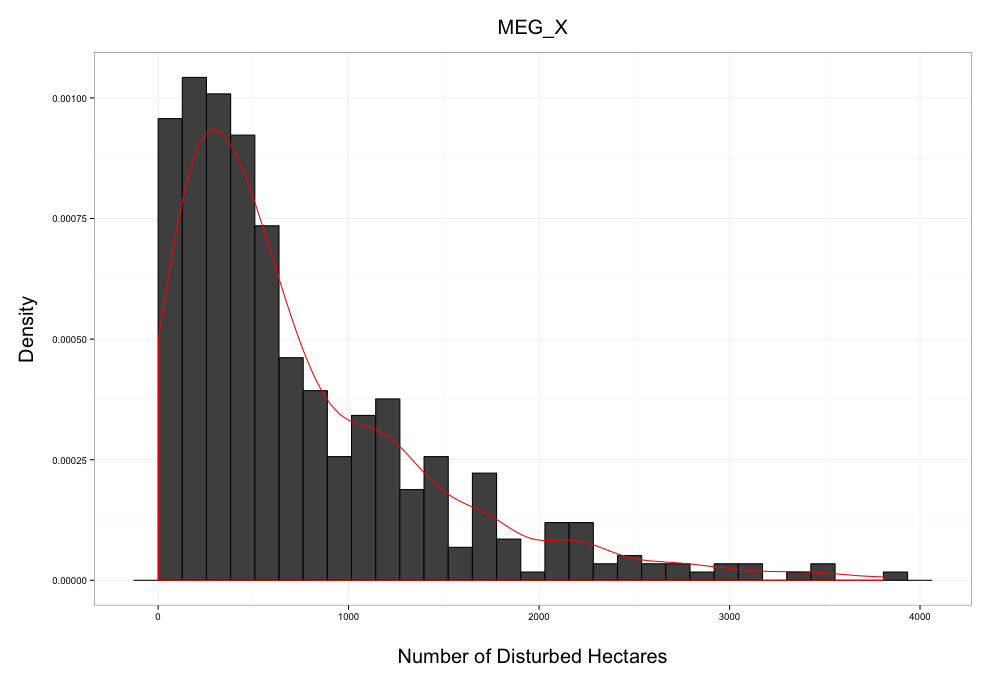
\includegraphics[width=0.5\textwidth]{/Users/mmallek/Tahoe/Report2/images/darea_hist_megx.png}
    }
  \caption{\small (a) Disturbance trajectory for Mixed Evergreen - Xeric. High mortality fire in dark blue; low mortality fire in light blue. (b) Histogram of disturbed hectares with density curve overlaid.} 
  \label{fig:darea_megx}
\end{figure}


Mixed Evergreen - Xeric (\textsc{meg\_x})is a somewhat common cover type within the core project area, encompassing 6,768 ha and comprising roughly 4\% of the project area. The frequency and extent of simulated wildfires in xeric mixed evergreen forest varied markedly across the landscape (Figure~\ref{fig:darea_megx} and Table~\ref{tab:darea_megx}). %
%
While xeric mixed evergreen forests always experienced some wildfire during the simulation, during a typical five year period wildfires burned across a larger extent on average than the mesic mixed evergreen forest, but the impacts were mostly low mortality. Low mortality fires were ten times as frequent as high mortality fires. Less than 1\% of the cover type (68 ha) burned during 6\% of the timesteps. Much more common were timesteps in which over 10\% of the landscape burned, which occurred about once in 13 years. The median proportion burned was 8\%. Seldom did large extents burn, at any mortality level, although roughly once every 46 years, more than 25\% of the cover type burned. Over 50\% of the landscape on very rare occasions (once in about 770 years). The maximum extent burned within the cover type was about 53\% (about 3,800 ha). %
%
Under this wildfire regime, the return interval between fires (of any mortality level) varied widely from 20 years to over 500 years, with a median of 48 years (Figure~\ref{fig:preturn_megm}). The median return interval and rotation values were influenced primarily by the dominant fire type, low mortality. Xeric mixed evergreen forests had a low mortality fire rotation of 51 years and a high mortality fire rotation of 472 years (Table~\ref{tab:darea_megm}).  %
%
In general, return intervals and canopy cover varied spatially across the forest and decreased with increasing TPI, reflecting our parameterization, which was based on the theory that higher, more southerly aspects are drier and more susceptible to fires. Canopy cover decreased by about 4\% when comparing minimum to maximum TPI (Table~\ref{tab:tpi_cc}).  %
%
Finally, when stands of xeric mixed evergreen forests were adjacent to cover types with shorter return intervals, they also exhibited shorter return intervals, reflecting the importance of landscape context on fire regimes.

%%%
The age structure and dynamics of xeric mixed evergreen forest illustrates the interaction between disturbance and succession processes. We focus our analysis on the 5$^{\text{th}}$ to 95$^{\text{th}}$ percentile range of variability for our simulation (excluding the equilibration period). %
%
The distribution of area among stand conditions within xeric mixed evergreen forest fluctuated over time (Figure~\ref{fig:covcond_megx}). Because high mortality fire is very rare in this cover type, and the time to reaching a Late Development stage is relatively short (Appendix~\ref{sec:covertypedesc}), the vast majority of the landscape, varying from 71\% to 87\%, was in the Late Development - Closed condition during the simulation (Table~\ref{tab:covcond1}).  %
%
The seral-stage distribution appeared to be in dynamic equilibrium (i.e., the percentage in each stand condition varied about a stable mean). Our calculated current seral-stage distribution was never observed under the simulated HRV (Table~\ref{tab:covcond1}). The most notable departure was the shift from Early and Mid Development to Late Development conditions. The current landscape contains 71\% of the xeric mixed evergreen forest in mid development conditions, but the late development conditions were always dominant under the simulated HRV. The current proportions of all mid development canopy cover levels are higher than at any point during the HRV. As described above, much of the shift from the dominance of mid development conditions observed in the current distribution to the dominance by late development conditions during the HRV can be attributed to the prodigious increase in the extent of Late Development - Closed (from 13\% to 71-87\%), although Late Development - Moderate was also well represented, with an HRV from 6\% to 15\%. The Early Development condition is also more common on the current landscape than during the simulation.

The spatial configuration of stand conditions fluctuated markedly over time as well, although there was considerable variation in the magnitude of variability among configuration metrics (Appendix \ref{sec:full-class-results}). Area-weighted patch and core area, patch density, and radius of gyration exhibited the greatest variability over time. Because the landscape is so dominated by the Late Development - Closed and Moderate canopy cover conditions, we can use their configuration metrics as a proxy for the landscape. In general, the current landscape contains fewer, smaller, and more isolated patches than existed under the simulated HRV. Patches in Late Development - Closed are less geometrically complex and have less area in cores in the current landscape than during the simulated HRV.


\begin{table}[!htbp]
\centering
\caption{\small Disturbed area summary statistics for Mixed Evergreen - Xeric. Proportions shown are relative to the total area of Mixed Evergreen - Xeric.}
\label{tab:darea_megx}
\begin{tabular}{@{}llll@{}}
\toprule
\textbf{\begin{tabular}[c]{@{}l@{}}Summary Statistic \\ (disturbed area/timestep)\end{tabular}} & \textbf{Low Mortality} & \textbf{High Mortality} & \textbf{Any Mortality} \\ \midrule
Minimum       & 0.04 		& 	0.00	& 0.04      \\
Maximum       & 52.63 		& 	8.30	& 56.30        \\
Median        & 6.79 		& 	0.63	& 7.56      \\
Mean          & 9.85 		& 	1.06	& 10.90       \\ 
\textbf{Fire Rotation} 	& 51 	& 472 	& 46 	\\ \bottomrule
\end{tabular}
\end{table}

%%%%%%%%%%%%%%%%%%%%%%%%%%%%%%%%%%%%%%%%%%%%%%%%%%%%%%%%%%%%%%%%%%%%%%%%%%%%%
%%%%%%%%%%%%%%%%%%%%%%%%%%%%%%%%%%%%%%%%%%%%%%%%%%%%%%%%%%%%%%%%%%%%%%%%%%%%%
%%%%%%%%%%%%%%%%%%%%%%%%%%%%%%%%%%%%%%%%%%%%%%%%%%%%%%%%%%%%%%%%%%%%%%%%%%%%%
%%%%%%%%%%%%%%%%%%%%%%%%%%%%%%%%%%%%%%%%%%%%%%%%%%%%%%%%%%%%%%%%%%%%%%%%%%%%%
%%%%%%%%%%%%%%%%%%%%%%%%%%%%%%%%%%%%%%%%%%%%%%%%%%%%%%%%%%%%%%%%%%%%%%%%%%%%%

%\clearpage
\section{Oak-Conifer Forest and Woodland} 

\begin{figure}[!htbp]
  \centering
  \subfloat[][]{
    \centering
    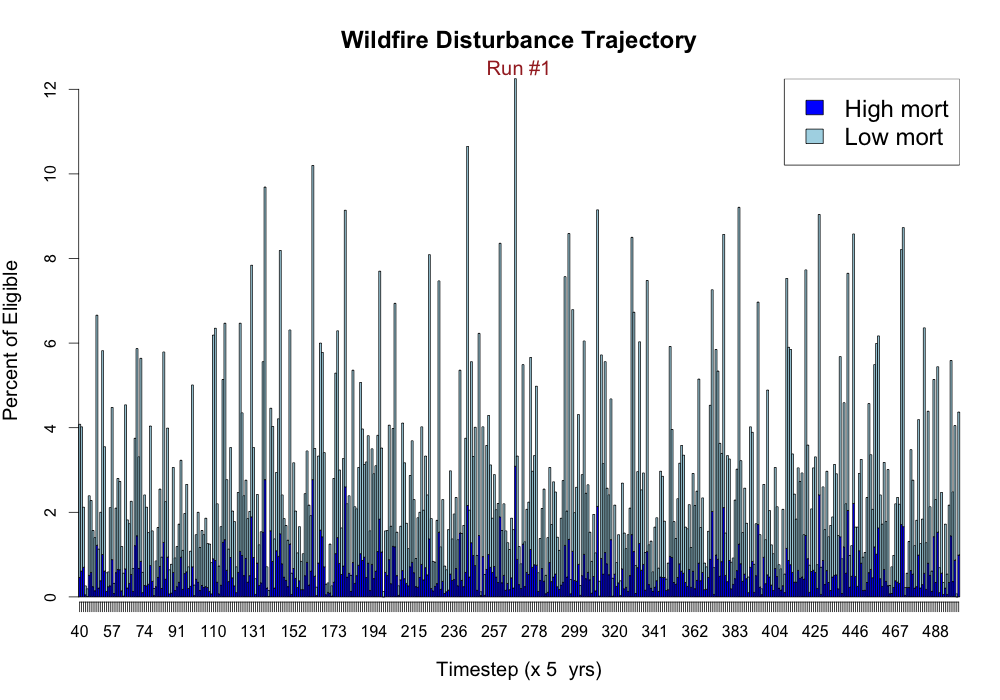
\includegraphics[width=0.5\textwidth]{/Users/mmallek/Tahoe/Report2/images/darea_ocfw.png}
    }%
  \subfloat[][]{
    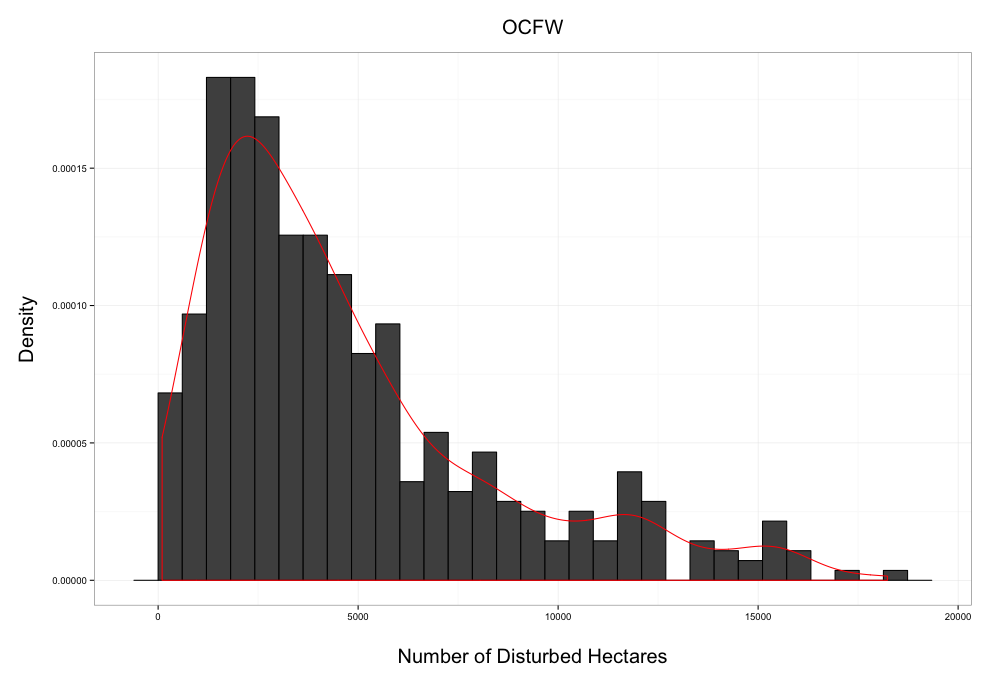
\includegraphics[width=0.5\textwidth]{/Users/mmallek/Tahoe/Report2/images/darea_hist_ocfw.png}
    }
  \caption{\small (a) Disturbance trajectory for Oak-Conifer Forest and Woodland. High mortality fire in dark blue; low mortality fire in light blue. (b) Histogram of disturbed hectares with density curve overlaid.} 
  \label{fig:darea_ocfw}
\end{figure}

Oak-Conifer Forest and Woodland (\textsc{ocfw})is the third most common cover type within the core project area, encompassing 23,279 ha and comprising roughly 13\% of the project area. The frequency and extent of simulated wildfires in oak-conifer forests and woodlands varied markedly across the landscape (Figure~\ref{fig:darea_ocfw} and Table~\ref{tab:darea_ocfw}).  %
%
Wildfire was quite prevalent in this cover type. At least some area burned every five years, and at least 10\% of the cover type burned in about 70\% of the simulated timesteps. The median amount of land burned during one timestep of the simulation was 15\%; over 25\% burned every 20 years. Wildfires occurred across more than 50\% of the cover type about once every 66 years. During one five year interval, nearly 80\% of the area in this type burned. The maximum extent burned within the cover type was about 78\% (18,200 ha). High mortality wildfire was about one-third as common as low mortality. %
%
Under this wildfire regime, the grand mean return interval between fires (of any mortality level) varied widely from 17 years to over 500 years, with a median of 25 years (Figure~\ref{fig:preturn_ocfw}). As expected, median return interval and rotation values are much shorter for this cover type as compared to the mixed evergreen forests, which occupy similar elevations. Like those forests, however, low mortality fire was the dominant type. Oak-conifer forests and woodlands had a low mortality fire rotation of 33 years and a high mortality fire rotation of 100 years. %
%
In general, return intervals and canopy cover varied spatially across the forest and decreased with increasing TPI, reflecting our parameterization, which was based on the theory that higher, more southerly aspects are drier and more susceptible to fires. Canopy cover decreased by about 8\% when comparing minimum to maximum TPI, from an average of 58\% to an average of 53\% (Table~\ref{tab:tpi_cc}). %
%
Finally, when stands of oak-conifer forests and woodland were adjacent to cover types with longer return intervals, they also exhibited longer return intervals, reflecting the importance of landscape context on fire regimes.
%%%

The age structure and dynamics of oak-conifer forests and woodlands illustrates the interaction between disturbance and succession processes. We focus our analysis on the 5$^{\text{th}}$ to 95$^{\text{th}}$ percentile range of variability for our simulation (excluding the equilibration period). %

The distribution of area among stand conditions within oak-conifer forests and woodlands fluctuated considerably over time, as expected (Figure~\ref{fig:covcond_ocfw}). For example, the percentage of oak-conifer forests and woodlands in the Late Development - Closed condition varied from 16\% to 38\%, reflecting the dynamic nature of this cover type (Table~\ref{tab:covcond1}). Surprisingly for a cover type in which fuels are the largest contributor to disturbance and fire is relatively frequent, the open canopy conditions were the least common of all condition classes, ranging from 6\%--15\% for Mid Development - Open and from 2\%--7\% for Late Development - Open. The other five condition classes were evenly distributed relative to each other. %
%
The seral-stage distribution appeared to be in dynamic equilibrium (i.e., the percentage in each stand condition varied about a stable mean). Our calculated current seral-stage distribution was never observed under the simulated HRV (Table~\ref{tab:covcond1}). The most notable departure was the shift from Mid Development conditions, which are dominant in the current landscape (76\%), to Late Development conditions, which are almost nonexistent on the current landscape (4\%). The current proportions of all Late Development canopy cover levels are lower than at any point during the HRV.  The Early Development condition is within the HRV ($76^{\text{th}}$ percentile), while the Mid Development - Moderate condition is just within the HRV ($94^{\text{th}}$ percentile).

The spatial configuration of stand conditions fluctuated markedly over time as well, although there was considerable variation in the magnitude of variability among configuration metrics (Appendix \ref{sec:full-class-results}). Area-weighted patch and core area exhibited the greatest variability over time. Because Late Development conditions are nearly absent from the current landscape, configuration metrics consistently differ between current conditions and the simulated HRV. The HRV results for class-level metrics are consistent for six of the seven condition classes, in the sense of their deviation from current conditions. For example, patches are currently smaller than during HRV, but tend to have larger core areas today. The quantity of patches is currently within the HRV, although during the simulation there were more in Late Development and fewer in Mid Development, which is consistent with our expectations based on the seral-stage distribution. Similarly, while patches are now geometrically less complex and more aggregated than the median simulated values, they are not necessarily outside the HRV.


\begin{table}[!htbp]
\centering
\caption{\small Disturbed area summary statistics for Oak-Conifer Forest and Woodland. Proportions shown are relative to the total area of Oak-Conifer Forest and Woodland.}
\label{tab:darea_ocfw}
\begin{tabular}{@{}llll@{}}
\toprule
\textbf{\begin{tabular}[c]{@{}l@{}}Summary Statistic \\ (disturbed area/timestep)\end{tabular}} & \textbf{Low Mortality} & \textbf{High Mortality} & \textbf{Any Mortality} \\ \midrule
Minimum       & 0.35	& 0.02	& 0.43      \\
Maximum       & 57.69	& 21.95	& 78.32         \\
Median        & 11.50	& 3.69	& 15.64       \\
Mean          & 15.14	& 5.00	& 20.14        \\ 
\textbf{Fire Rotation} & 33	& 100	& 25 \\ \bottomrule
\end{tabular}
\end{table}


%%%%%%%%%%%%%%%%%%%%%%%%%%%%%%%%%%%%%%%%%%%%%%%%%%%%%%%%%%%%%%%%%%%%%%%%%%%%%
%%%%%%%%%%%%%%%%%%%%%%%%%%%%%%%%%%%%%%%%%%%%%%%%%%%%%%%%%%%%%%%%%%%%%%%%%%%%%
%%%%%%%%%%%%%%%%%%%%%%%%%%%%%%%%%%%%%%%%%%%%%%%%%%%%%%%%%%%%%%%%%%%%%%%%%%%%%
%%%%%%%%%%%%%%%%%%%%%%%%%%%%%%%%%%%%%%%%%%%%%%%%%%%%%%%%%%%%%%%%%%%%%%%%%%%%%
%%%%%%%%%%%%%%%%%%%%%%%%%%%%%%%%%%%%%%%%%%%%%%%%%%%%%%%%%%%%%%%%%%%%%%%%%%%%%
%\clearpage
\section{Oak-Conifer Forest and Woodland - Ultramafic} 

\begin{figure}[!htbp]
  \centering
  \subfloat[][]{
    \centering
    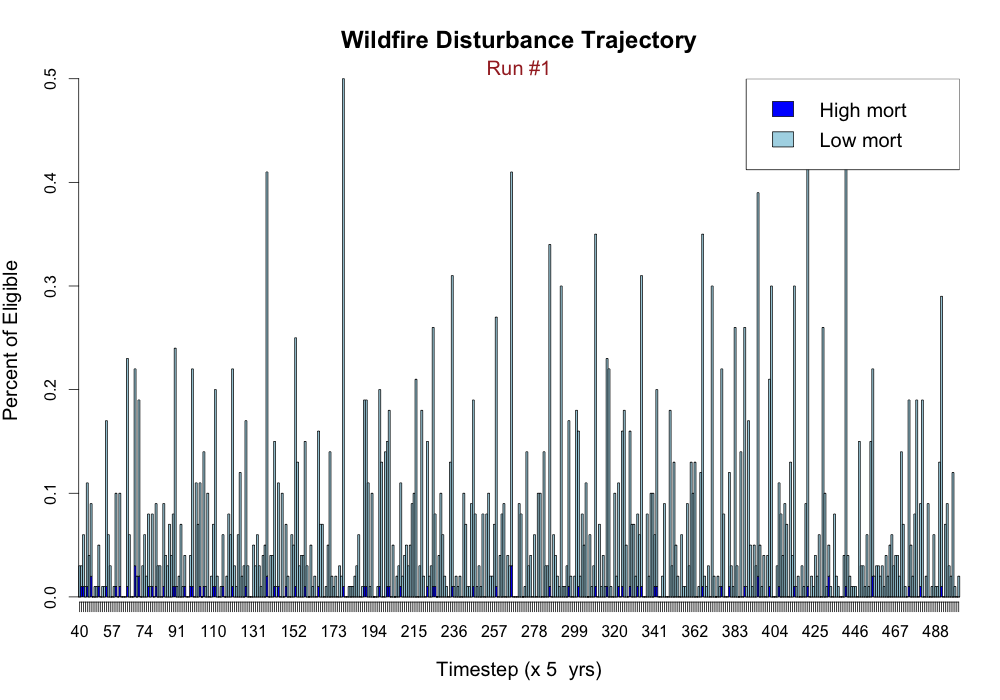
\includegraphics[width=0.5\textwidth]{/Users/mmallek/Tahoe/Report2/images/darea_ocfwu.png}
    }%
  \subfloat[][]{
    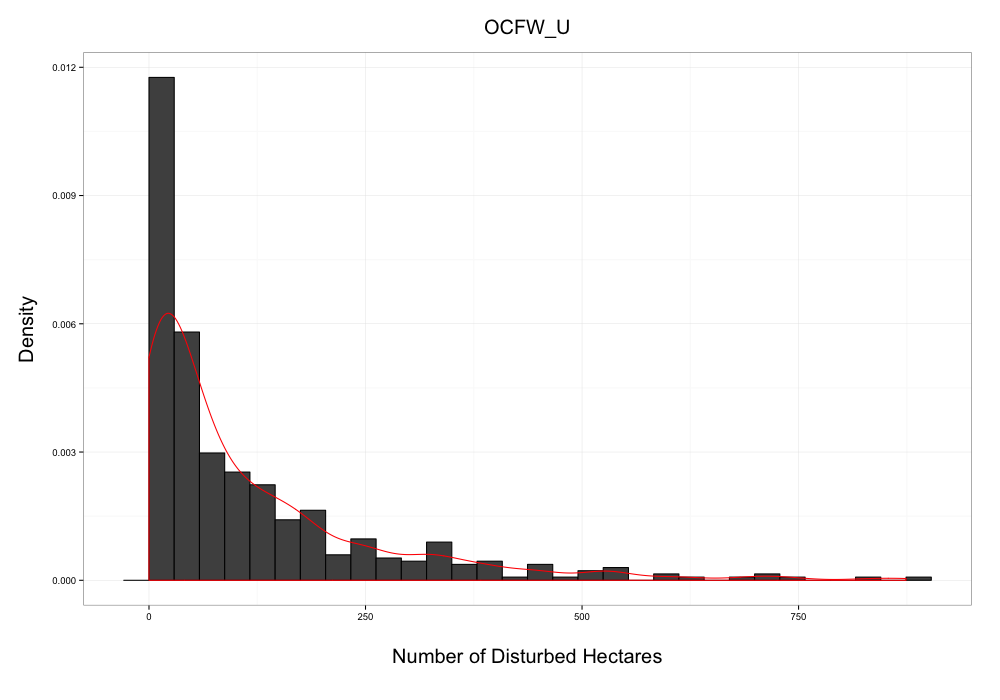
\includegraphics[width=0.5\textwidth]{/Users/mmallek/Tahoe/Report2/images/darea_hist_ocfwu.png}
    }
  \caption{\small (a) Disturbance trajectory for Oak-Conifer Forest and Woodland - Ultramafic. High mortality fire in dark blue; low mortality fire in light blue. (b) Histogram of disturbed hectares with density curve overlaid.} 
  \label{fig:darea_ocfwu}
\end{figure}

Oak-Conifer Forest and Woodland - Ultramafic (\textsc{ocfw\_u})is a relatively uncommon cover type within the core project area, encompassing 1,060 ha and comprising roughly 0.6\% of the project area. The frequency and extent of simulated wildfires in ultramafic oak-conifer forests and woodlands varied markedly across the landscape (Figure~\ref{fig:darea_ocfwu} and Table~\ref{tab:darea_ocfwu}). %
%
Wildfire is much less common in this cover type compared to its non-ultramafic oak-conifer forests and woodlands. Ultramafic soils support scattered, but rarely dense stands of trees and shrubs, creating fuel discontinuities that stop fires from spreading easily. All ultramafic oak-conifer forests and woodlands escaped fire 14 times during the simulation, and less than 1\% (11 ha) of them burned during 21\% of the timesteps. Much of this is due to the extreme rarity of high mortality fire, which never burned more than 5\% of this cover type, and actually averaged 0.42\% high mortality. In contrast, low mortality fire was fairly common, and over 10\% of the landscape burned about once every 14 years, predominantly as low mortality fire. The median proportion burned was 5\%. Selcom did large extents burn, although once every 40 years more than 25\% of the cover type burned.Fires spread over 50\% of the cover type only once every 192 years. Low mortality wildfire was nearly 25 times as common as high mortality. %
%
Under this wildfire regime, the grand mean return interval between fires (of any mortality level) varied widely from 21 years to over 500 years, with a median of 48 years (Figure~\ref{fig:preturn_ocfwu}). As expected, median return interval and rotation values are much longer for this cover type compared to the non-ultramafic variant (Table~\ref{tab:darea_ocfw}), and were clearly influenced by the dominant fire type, low mortality. Ultramafic oak-conifer forests and woodlands had a low mortality fire rotation of 48 years and a high mortality fire rotation of 1192 years (Table~\ref{tab:darea_ocfwu}).  %
%
Return intervals and canopy cover varied spatially across the ultramafic oak-conifer forests and woodlands, as expected, and increased with increasing TPI, which was not predicted. Canopy cover increased by about 3\% when comparing minimum to maximum TPI, the only focal cover type for which we observed an increase (Table~\ref{tab:tpi_cc}). 


%%%
The age structure and dynamics of ultramafic oak-conifer forests and woodlands illustrates the interaction between disturbance and succession processes. We focus our analysis on the 5$^{\text{th}}$ to 95$^{\text{th}}$ percentile range of variability for our simulation (excluding the equilibration period). %
%
The distribution of area among stand conditions within ultramafic oak-conifer forests and woodlands did not appear to reach equilibrium until approximately timestep 220 (Figure~\ref{fig:covcond_ocfwu}). When it did reach equilibrium, the vast majority of the cover type was in the Late Development - Open condition. It ranged from 46\%--93\%, but because the equilibration period for this cover type was so long, it may be more instructive to consider the $25^{\text{th}}$--$75^{\text{th}}$ percentile range, which is 81\%--91\%. This is consistent with the extremely low rate of high mortality fire just described, which is required to re-initiate a stand in our model. Consequently, the resulting condition class distribution was dramatically different from the current distribution, which is primarily composed of Middle Development conditions. All conditions except Late Development - Moderate were well outside the HRV. %
%
The seral-stage distribution appeared to eventually reach a dynamic equilibrium (i.e., the percentage in each stand condition varied about a stable mean). Our calculated current seral-stage distribution was never observed under the simulated HRV (Table~\ref{tab:covcond1}). The most striking departure was the dramatic shift away from all conditions to Late Development - Open. Currently, Late Development - Open extends across just 0.34\% of the cover type. 

The spatial configuration of stand conditions fluctuated markedly over time as well, although there was considerable variation in the magnitude of variability among configuration metrics (Appendix \ref{sec:full-class-results}). Area-weighted patch and core area, patch density, mean similarity, and radius of gyration all exhibited high variability over time. For the most part, the current landscape's values fall within the HRV. Patches and their cores are larger, more complex, and more numerous compared to the median for the simulated HRV. The current landscape also has more aggregated patches. However, we caution against drawing firm conclusions, since this type did not reach equilibrium until halfway through the simulation.

\begin{table}[!htbp]
\centering
\caption{\small Disturbed area summary statistics for Oak-Conifer Forest and Woodland - Ultramafic. Proportions shown are relative to the total area of Oak-Conifer Forest and Woodland - Ultramafic.}
\label{tab:darea_ocfwu}
\begin{tabular}{@{}llll@{}}
\toprule
\textbf{\begin{tabular}[c]{@{}l@{}}Summary Statistic \\ (disturbed area/timestep)\end{tabular}} & \textbf{Low Mortality} & \textbf{High Mortality} & \textbf{Any Mortality} \\ \midrule
Minimum       & 0.00	&   0.00	& 0.00     \\
Maximum       & 80.35	&   4.28	& 82.46        \\
Median        & 5.02	&   0.14	& 5.26     \\
Mean          & 10.34	&   0.42	& 10.76       \\ 
\textbf{Fire Rotation} & 48	& 1192	& 46 \\ \bottomrule
\end{tabular}
\end{table}

%%%%%%%%%%%%%%%%%%%%%%%%%%%%%%%%%%%%%%%%%%%%%%%%%%%%%%%%%%%%%%%%%%%%%%%%%%%%%
%%%%%%%%%%%%%%%%%%%%%%%%%%%%%%%%%%%%%%%%%%%%%%%%%%%%%%%%%%%%%%%%%%%%%%%%%%%%%
%%%%%%%%%%%%%%%%%%%%%%%%%%%%%%%%%%%%%%%%%%%%%%%%%%%%%%%%%%%%%%%%%%%%%%%%%%%%%
%%%%%%%%%%%%%%%%%%%%%%%%%%%%%%%%%%%%%%%%%%%%%%%%%%%%%%%%%%%%%%%%%%%%%%%%%%%%%
%%%%%%%%%%%%%%%%%%%%%%%%%%%%%%%%%%%%%%%%%%%%%%%%%%%%%%%%%%%%%%%%%%%%%%%%%%%%%
%\clearpage
\section{Red Fir - Mesic} 

\begin{figure}[!htbp]
  \centering
  \subfloat[][]{
    \centering
    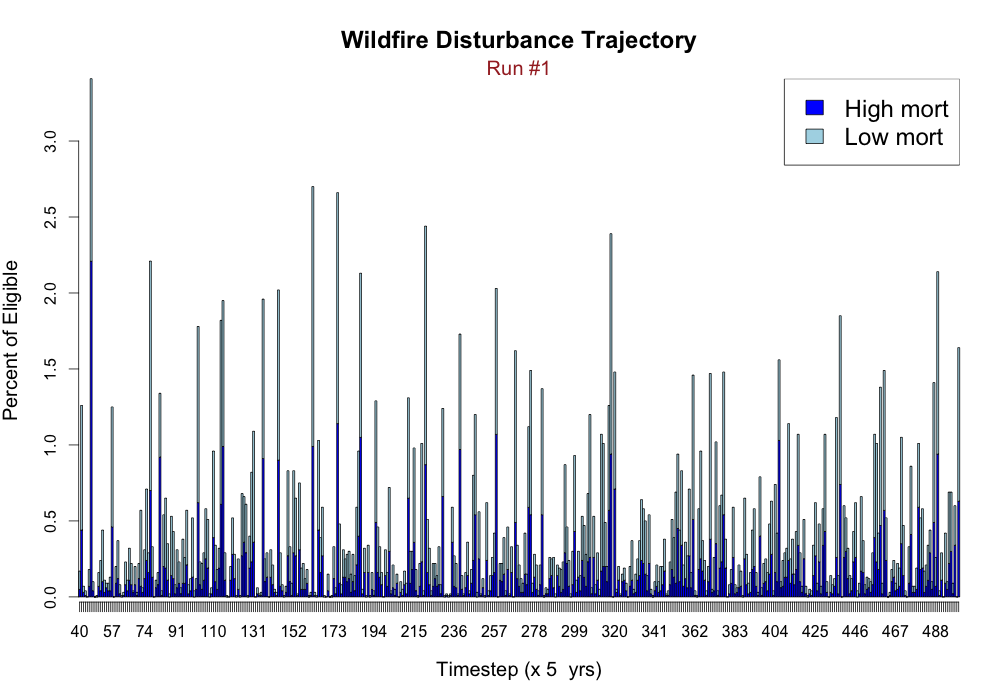
\includegraphics[width=0.5\textwidth]{/Users/mmallek/Tahoe/Report2/images/darea_rfrm.png}
    }%
  \subfloat[][]{
    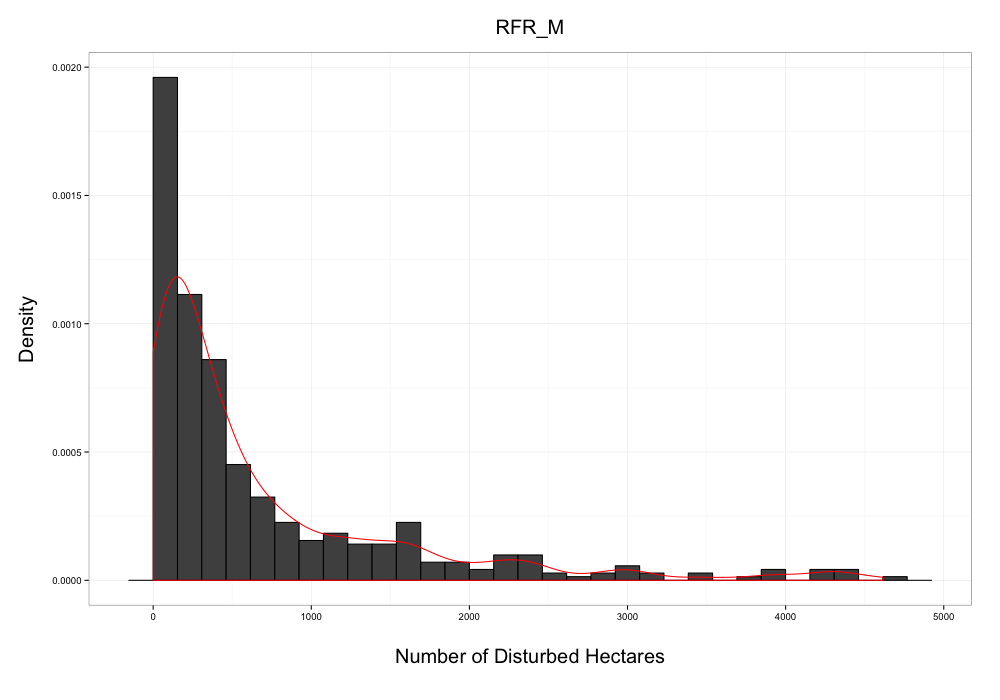
\includegraphics[width=0.5\textwidth]{/Users/mmallek/Tahoe/Report2/images/darea_hist_rfrm.png}
    }
  \caption{\small (a) Disturbance trajectory for Red Fir - Mesic. High mortality fire in dark blue; low mortality fire in light blue. (b) Histogram of disturbed hectares with density curve overlaid.} 
  \label{fig:darea_rfrm}
\end{figure}

Red Fir - Mesic (\textsc{rfr\_m})is a somewhat common cover type within the core project area, encompassing 8,563 ha and comprising roughly 5\% of the project area. The frequency and extent of simulated wildfires in mesic red fir forests varied markedly across the landscape (Figure~\ref{fig:darea_rfrm} and Table~\ref{tab:darea_rfrm}). %
%
Wildfire was fairly common in this cover type. At least some area in mesic red fir forests burned during each timestep in the simulation, although in 20\% of these less than 1\% of the cover type (86 ha) burned. When fires did occur they were seldom very large. At least 10\% of these forests burned about once every 20 years, and fires burned over 25\% of the cover type once in 60 years. However, over wildfires spread over 50\% of the cover type only once in 576 years. The maximum extent burned was 54\% (4,600 ha). The median and mean area burned was 4\% and 8\%, respectively. Low mortality fire was roughly 1.5 times as likely to occur as high mortality fire. %
%
Under this wildfire regime, the grand mean return interval between fires (of any mortality level) varied widely from 21 years to over 500 years, with a median of 68 years (Figure~\ref{fig:preturn_rfrm}). Median return interval and rotation values tend to be longer in red fir forests compared to sierran mixed conifer forests, because their higher elevation corresponds to cooler and moister conditions. Mesic red fir forests had a low mortality fire rotation of 101 years and a high mortality fire rotation of 164 years (Table~\ref{tab:darea_rfrm}); neither high nor low mortality fires dominate the cover type.  %
%
In general, return intervals and canopy cover varied spatially across the forest and decreased with increasing TPI, reflecting our parameterization, which was based on the theory that higher, more southerly aspects are drier and more susceptible to fires. Canopy cover decreased by about 11\% when comparing minimum to maximum TPI, from an average of 72\% to an average of 64\% (Table~\ref{tab:tpi_cc}).  %
%
Finally, when stands of mesic red fir forests were adjacent to cover types with much shorter or longer return intervals, they also exhibited a directional shift in local return intervals towards that of the adjacent type, reflecting the importance of landscape context on fire regimes.

%%%
The age structure and dynamics of mesic red fir forests illustrates the interaction between disturbance and succession processes. We focus our analysis on the 5$^{\text{th}}$ to 95$^{\text{th}}$ percentile range of variability for our simulation (excluding the equilibration period). %
%
The distribution of area among stand conditions within mesic red fir forests fluctuated considerably over time (Figure~\ref{fig:covcond_rfrm}). For example, the percentage of mesic red fir forests in the Early Development condition varied from 7\% to 32\%, reflecting the dynamic nature of this cover type (Table~\ref{tab:covcond2}). As expected for mesic red fir forests (Appendix~\ref{sec:covertypedesc}), closed canopy conditions predominated. The proportion of the cover type occupied by Mid Development - Closed ranged from 21\%--49\% (currently at 4\%) and the proportion occupied by Late Development - Closed ranged from 28\%--54\% (currently at 11\%). The shift towards closed canopies when stands reached the Late Development stage may be due to an increasing resilience to wildfire disturbances by stands of that age: wildfires may burn the understory without significantly affecting overstory canopy cover. Early Development, which includes post-fire chaparral fields, was the next most extensive cover type. %
%
The seral-stage distribution appeared to be in dynamic equilibrium (i.e., the percentage in each stand condition varied about a stable mean). Our calculated current seral-stage distribution was never observed under the simulated HRV (Table~\ref{tab:covcond2}). The most notable departure was a shift from moderate canopy cover to closed canopy cover. Current levels of moderate canopy cover are much higher (41\%), and current levels of closed canopy cover much lower (14\%), than during the simulated HRV. Early Development and Late Development - Open are both within the HRV at the $79^{\text{th}}$ and $87^{\text{th}}$ percentiles, respectively. The current proportions of all late development canopy cover levels are lower than at any point during the HRV.  The Early Development condition is within the HRV ($76^{\text{th}}$ percentile). The Mid Development - Moderate condition is just within it ($94^{\text{th}}$ percentile).

The spatial configuration of stand conditions fluctuated markedly over time as well, although there was considerable variation in the magnitude of variability among configuration metrics (Appendix \ref{sec:full-class-results}). Several metrics exhibited high variability over time, including the area-weighted patch and core area, edge and patch density, radius of gyration, and contrast-weighted edge density. In general, current values for the class metrics are usually outside of the simulated HRV. Specifically, current patches tend to be smaller in both area and core area and more numerous. They also have more complex geometries and more edge than patches during the simulated HRV.

\begin{table}[!htbp]
\centering
\caption{\small Disturbed area summary statistics for Red Fir - Mesic. Proportions shown are relative to the total area of Red Fir - Mesic.}
\label{tab:darea_rfrm}
\begin{tabular}{@{}llll@{}}
\toprule
\textbf{\begin{tabular}[c]{@{}l@{}}Summary Statistic \\ (disturbed area/timestep)\end{tabular}} & \textbf{Low Mortality} & \textbf{High Mortality} & \textbf{Any Mortality} \\ \midrule
Minimum       & 0.01	& 	0.00	& 0.01       \\
Maximum       & 42.67	& 	28.02	& 53.90         \\
Median        & 2.36	& 	1.31	& 3.88       \\
Mean          & 4.95	& 	3.06	& 8.01        \\ 
\textbf{Fire Rotation} & 101	& 164	& 62 \\ \bottomrule
\end{tabular}
\end{table}


%%%%%%%%%%%%%%%%%%%%%%%%%%%%%%%%%%%%%%%%%%%%%%%%%%%%%%%%%%%%%%%%%%%%%%%%%%%%%
%%%%%%%%%%%%%%%%%%%%%%%%%%%%%%%%%%%%%%%%%%%%%%%%%%%%%%%%%%%%%%%%%%%%%%%%%%%%%
%%%%%%%%%%%%%%%%%%%%%%%%%%%%%%%%%%%%%%%%%%%%%%%%%%%%%%%%%%%%%%%%%%%%%%%%%%%%%
%%%%%%%%%%%%%%%%%%%%%%%%%%%%%%%%%%%%%%%%%%%%%%%%%%%%%%%%%%%%%%%%%%%%%%%%%%%%%
%%%%%%%%%%%%%%%%%%%%%%%%%%%%%%%%%%%%%%%%%%%%%%%%%%%%%%%%%%%%%%%%%%%%%%%%%%%%%
%\clearpage
\section{Red Fir - Xeric} 

\begin{figure}[!htbp]
  \centering
  \subfloat[][]{
    \centering
    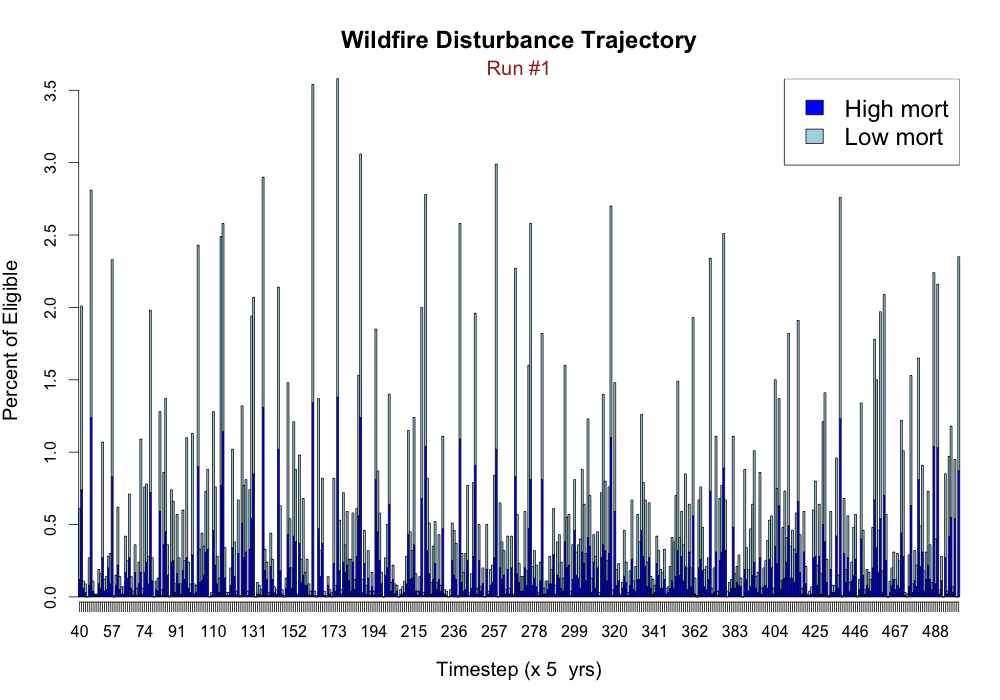
\includegraphics[width=0.5\textwidth]{/Users/mmallek/Tahoe/Report2/images/darea_rfrx.png}
    }%
  \subfloat[][]{
    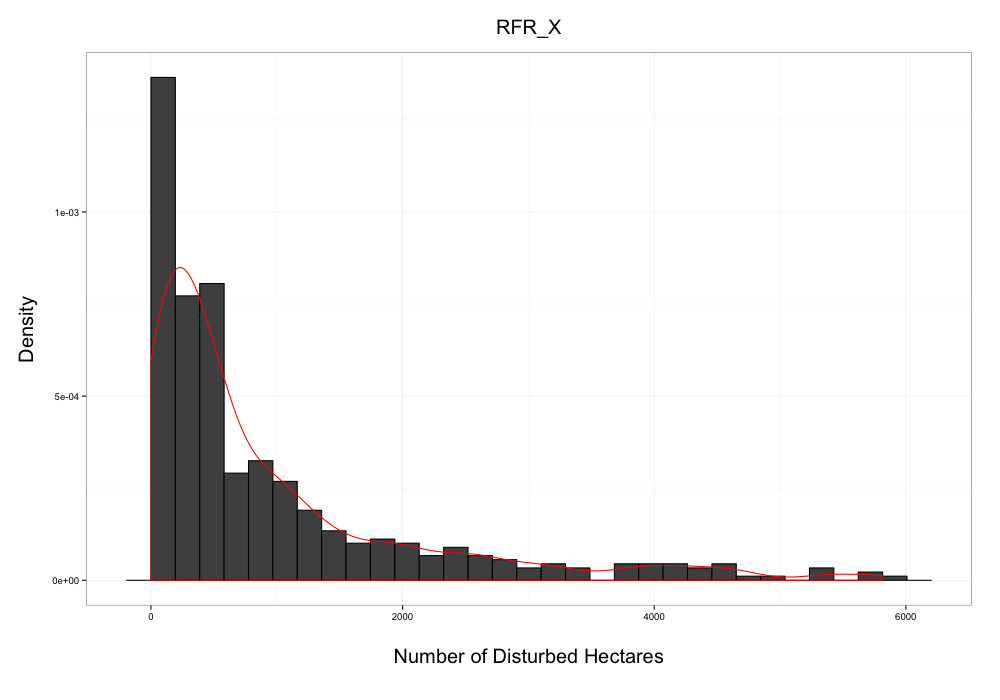
\includegraphics[width=0.5\textwidth]{/Users/mmallek/Tahoe/Report2/images/darea_hist_rfrx.png}
    }
  \caption{\small (a) Disturbance trajectory for Red Fir - Xeric. High mortality fire in dark blue; low mortality fire in light blue. (b) Histogram of disturbed hectares with density curve overlaid.} 
  \label{fig:darea_rfrx}
\end{figure}

Red Fir - Xeric (\textsc{rfr\_x})is a somewhat common cover type within the core project area, encompassing 7,493 ha and comprising roughly 5\% of the project area. The frequency and extent of simulated wildfires in xeric red fir forests varied markedly across the landscape (Figure~\ref{fig:darea_rfrx} and Table~\ref{tab:darea_rfrx}). %
%
Wildfire was fairly common in this cover type, and occurred more frequently on average than in mesic red fir forests. Xeric red fir forests burned during every timestep, and during a typical five-year period 8--10\% of the cover type burned. The disturbed area per timestep varied dramatically, from a minimum of 0.02\% to a maximum of 78\% (about 5,800 ha). More than 10\% of xeric red fir forest extent burned at about a 13 year interval, more than 25\% burned at a 60 year interval, and fires burning over 50\% of the cover type occured once in 90 years. Low mortality fire was twice as likely as high mortality fire. %
%
Under this wildfire regime, the grand mean return interval between fires (of any mortality level) varied widely from 20 years to over 500 years, with a median of 40 years (Figure~\ref{fig:preturn_rfrx}). Median return interval and rotation values tend to be longer in red fir forests compared to sierran mixed conifer forests, because their higher elevation corresponds to cooler and moister conditions. Xesic red fir forests had a low mortality fire rotation of 59 years and a high mortality fire rotation of 117 years (Table~\ref{tab:darea_rfrx}). These values are shorter in xeric red fir compared to mesic red fir, but much longer than oak-conifer or sierran mixed conifer forests, which occur at lower elevations. %
%
In general, return intervals and canopy cover varied spatially across the forest and decreased with increasing TPI, reflecting our parameterization, which was based on the theory that higher, more southerly aspects are drier and more susceptible to fires. Canopy cover decreased by about 29\% when comparing minimum to maximum TPI, from an average of 41\% to an average of 29\% (Table~\ref{tab:tpi_cc}). %
%
Finally, when stands of xeric red fir forests were adjacent to cover types with much shorter or longer return intervals, they also exhibited a directional shift in local return intervals towards that of the adjacent type, reflecting the importance of landscape context on fire regimes.

%%%
The age structure and dynamics of xeric red fir forests reflected the interplay between disturbance and succession processes. We focus our analysis on the 5$^{\text{th}}$ to 95$^{\text{th}}$ percentile range of variability for our simulation (excluding the equilibration period). %
%
The distribution of area among stand conditions within xeric red fir forests fluctuated considerably over time, as expected (Figure~\ref{fig:covcond_rfrx}). For example, the percentage of xeric red fir forests in the Early Development condition varied from 27\% to 48\%, reflecting the dynamic nature of this cover type (Table~\ref{tab:covcond2}). Interestingly, although open canopy conditions dominated during middle development, the distribution of the three late development canopy conditions was roughly even. The shift towards higher canopy closure as stands reached the Late Development stage may be due to an increasing resilience to wildfire disturbances by stands of that age: wildfires may burn the understory without significantly affecting overstory canopy cover. Early Development, which includes post-fire chaparral fields, was the single most extensive cover type. The current proportion of Early Development is easily within the simulated HRV, in the 32$^{\text{nd}}$ percentile. %
%
The seral-stage distribution appeared to be in dynamic equilibrium (i.e., the percentage in each stand condition varied about a stable mean). Our calculated current seral-stage distribution was never observed under the simulated HRV (Table~\ref{tab:covcond2}). The most notable departure was a reduction in moderate and closed canopy cover and an increase in open canopy cover within the Mid Development stage. Current levels of moderate and closed canopy cover are much higher than ever observed during the simulated HRV. Late Development - Closed and Moderate are both within the HRV at the $35^{\text{th}}$ and $59^{\text{th}}$ percentiles, respectively. Late Development - Open is currently fairly rare on the landscape (3\%), but more common during the simulated HRV (7\%--15\%). 

The spatial configuration of stand conditions fluctuated markedly over time as well, although there was considerable variation in the magnitude of variability among configuration metrics (Appendix \ref{sec:full-class-results}). Area-weighted patch and core area exhibited the most variability over time. In general, current values for the class metrics are often completely outside or near the extremes of the simulated HRV. Specifically, current patches tend to be smaller in both area and core area and more numerous, with less complex geometries and more edge than patches during the simulated HRV.

\begin{table}[!htbp]
\centering
\caption{\small Disturbed area summary statistics for Red Fir - Xeric. Proportions shown are relative to the total area of Red Fir - Xeric.}
\label{tab:darea_rfrx}
\begin{tabular}{@{}llll@{}}
\toprule
\textbf{\begin{tabular}[c]{@{}l@{}}Summary Statistic \\ (disturbed area/timestep)\end{tabular}} & \textbf{Low Mortality} & \textbf{High Mortality} & \textbf{Any Mortality} \\ \midrule
Minimum       & 0.02	& 	0.00	& 0.02   \\
Maximum       & 52.49	& 	31.50	& 77.63       \\
Median        & 4.49	& 	2.07	& 6.55   \\
Mean          & 8.49	& 	4.27	& 12.76     \\ 
\textbf{Fire Rotation} & 59	& 117	& 39 \\ \bottomrule
\end{tabular}
\end{table}


%%%%%%%%%%%%%%%%%%%%%%%%%%%%%%%%%%%%%%%%%%%%%%%%%%%%%%%%%%%%%%%%%%%%%%%%%%%%%
%%%%%%%%%%%%%%%%%%%%%%%%%%%%%%%%%%%%%%%%%%%%%%%%%%%%%%%%%%%%%%%%%%%%%%%%%%%%%
%%%%%%%%%%%%%%%%%%%%%%%%%%%%%%%%%%%%%%%%%%%%%%%%%%%%%%%%%%%%%%%%%%%%%%%%%%%%%
%%%%%%%%%%%%%%%%%%%%%%%%%%%%%%%%%%%%%%%%%%%%%%%%%%%%%%%%%%%%%%%%%%%%%%%%%%%%%
%%%%%%%%%%%%%%%%%%%%%%%%%%%%%%%%%%%%%%%%%%%%%%%%%%%%%%%%%%%%%%%%%%%%%%%%%%%%%
%\clearpage
\section{Sierran Mixed Conifer - Mesic} 

\begin{figure}[!htbp]
  \centering
  \subfloat[][]{
    \centering
    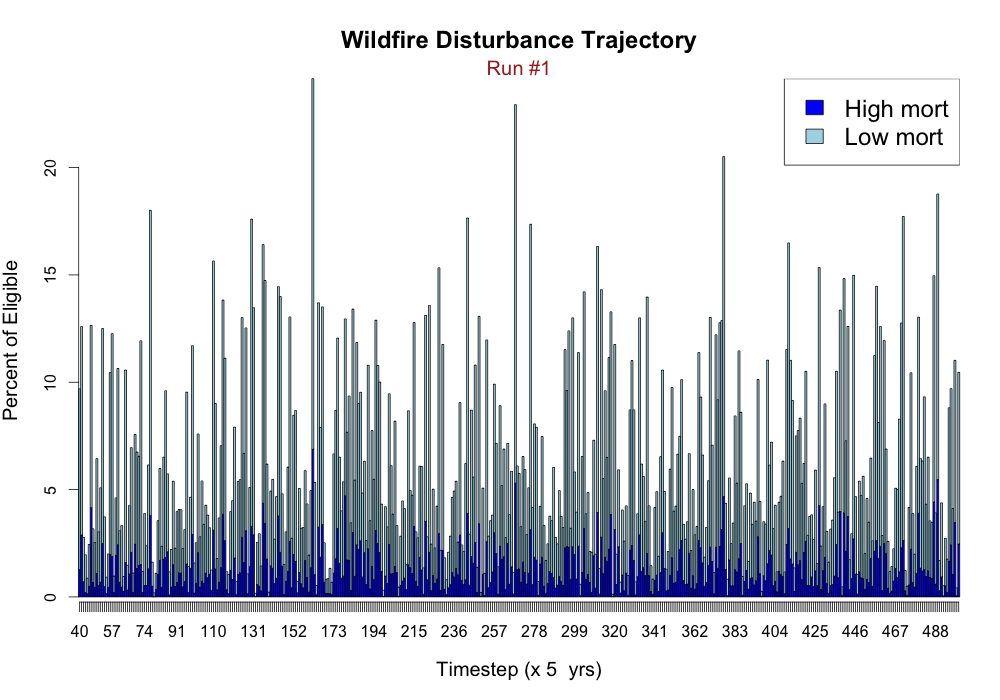
\includegraphics[width=0.5\textwidth]{/Users/mmallek/Tahoe/Report2/images/darea_smcm.png}
    }%
  \subfloat[][]{
    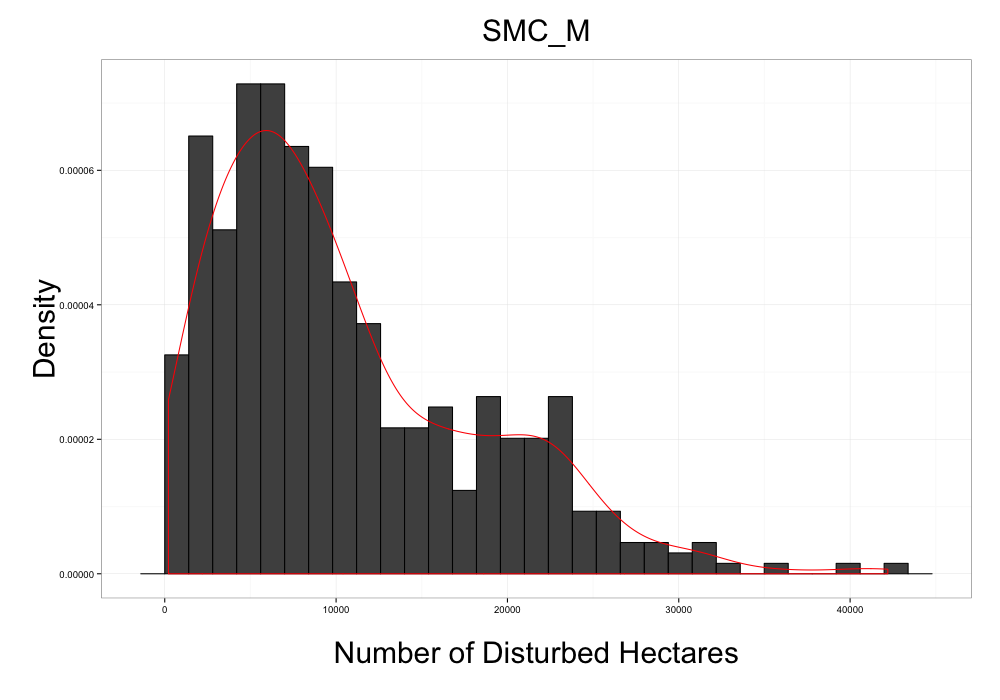
\includegraphics[width=0.5\textwidth]{/Users/mmallek/Tahoe/Report2/images/darea_hist_smcm.png}
    }
  \caption{\small (a) Disturbance trajectory for Sierran Mixed Conifer - Mesic. High mortality fire in dark blue; low mortality fire in light blue. (b) Histogram of disturbed hectares with density curve overlaid.} 
  \label{fig:darea_smcm}
\end{figure}

Sierran Mixed Conifer - Mesic (\textsc{smc\_m}) is the dominant cover type within the core project area, encompassing 57,853 ha and comprising roughly 32\% of the project area. The frequency and extent of simulated wildfires in sierran mixed conifer forests varied markedly across the landscape (Figure~\ref{fig:darea_smcm} and Table~\ref{tab:darea_smcm}). %
%
Wildfire was prevalent in this cover type. At least some area burned every five years, and at least 10\% of the cover type burned in 64\% of the simulated timesteps. The median amount of land burned during on timestep was 13\%. Over 25\% burned at a 20 year interval. Wildfires that extended across large extents of mesic mixed conifer forests were infrequent; at least 50\% of the cover type burned only once every 210 years. There was tremendous variability in the amount of area burned, from a minimum of 0.2\% to a maximum of 72\% (over 41,500 ha). Low mortality fires, the dominant disturbance type on these forests, are roughly three times as common as high mortality fires. %
%
Under this wildfire regime, the grand mean return interval between fires (of any mortality level) varied widely from 18 years to over 500 years, with a median of 29 years (Figure~\ref{fig:preturn_smcm}). Median return interval and rotation values tend to be shorter in mixed conifer forests than in red fir forests, because their lower elevation corresponds to warmer and drier conditions. Mesic mixed conifer forests had a low mortality fire rotation of 39 years and a high mortality fire rotation of 115 years (Table~\ref{tab:darea_smcm}).  %
%
In general, return intervals and canopy cover varied spatially across the forest and decreased with increasing TPI, reflecting our parameterization, which was based on the theory that higher, more southerly aspects are drier and more susceptible to fires. Canopy cover decreased by about 9\% when comparing minimum to maximum TPI (Table~\ref{tab:tpi_cc}).  %
%
Finally, when stands of mesic sierran mixed conifer forests were adjacent to cover types with much shorter or longer return intervals, they also exhibited a directional shift in local return intervals towards that of the adjacent type, reflecting the importance of landscape context on fire regimes.

%%%
The age structure and dynamics of mesic mixed conifer forests illustrates the interaction between disturbance and succession processes. We focus our analysis on the 5$^{\text{th}}$ to 95$^{\text{th}}$ percentile range of variability for our simulation (excluding the equilibration period). %
%
The distribution of area among stand conditions within mesic mixed conifer forests fluctuated over time, as expected (Figure~\ref{fig:covcond_smcm}). For example, the percentage of mesic mixed conifer forests in the Early Development condition varied from 8\%--20\%, reflecting the dynamic nature of this cover type (Table~\ref{tab:covcond2}). This condition is currently within the simulated HRV (47$^{\text{th}}$ percentile). Mid Development - Closed was typically the most extensive condition class (20\%-37\%), but most of the condition classes were common throughout the simulation. The shift towards closed canopies when stands reached the Late Development stage may be due to an increasing resilience to wildfire disturbances by stands of that age: wildfires may burn the understory without significantly affecting overstory canopy cover. %
%
The seral-stage distribution appeared to be in dynamic equilibrium (i.e., the percentage in each stand condition varied about a stable mean). Our calculated current seral-stage distribution was never observed under the simulated HRV (Table~\ref{tab:covcond2}). The most notable departure was an increase in Mid Development - Closed extent and a decrease in Mid and Late Development - Moderate extent during the simulated HRV; these condition classes are currently all outside of the simulated HRV. The other two Late Development classes are within the HRV, with the closed canopy and open canopy conditions currently in the $76^{\text{th}}$ and $41^{\text{st}}$ percentiles, respectively. Late Development - Open is the least common condition on the landscape during both the HRV and today.

The spatial configuration of stand conditions fluctuated markedly over time as well, although there was considerable variation in the magnitude of variability among configuration metrics (Appendix \ref{sec:full-class-results}). Area-weighted patch and core area, and radius of gyration, exhibited the greatest variability over time. The class-level metrics for mesic mixed conifer forests do not consistently diverge from the HRV in one direction, nor are all classes outside the simulated HRV for our focal metrics. Instead, we observe that, for example, there are shifts in which patches have large extents: Early Development patches were much larger during the HRV, but Late Development - Moderate patches were smaller. We observed a similar pattern for core area and for \emph{Shape}. The current values indicate that Early Development patches are less geometrically complex, and Late Development - Moderate patches more geometrically complex, than during the simulated HRV. Early development and Mid Development - Closed are currently less aggregated than during the simulated HRV, but the remaining condition classes were more aggregated. Thus no clear pattern emerges within the mesic mixed conifer cover type regarding departure from the HRV.


\begin{table}[!htbp]
\centering
\caption{\small Disturbed area summary statistics for Sierran Mixed Conifer - Mesic. Proportions shown are relative to the total area of Sierran Mixed Conifer - Mesic.}
\label{tab:darea_smcm}
\begin{tabular}{@{}llll@{}}
\toprule
\textbf{\begin{tabular}[c]{@{}l@{}}Summary Statistic \\ (disturbed area/timestep)\end{tabular}} & \textbf{Low Mortality} & \textbf{High Mortality} & \textbf{Any Mortality} \\ \midrule
Minimum       & 0.18	& 	0.02	& 0.20      \\
Maximum       & 49.19	& 	23.53	& 71.76         \\
Median        & 10.16	& 	3.23	& 13.40       \\
Mean          & 12.95	& 	4.37	& 17.32        \\ 
\textbf{Fire Rotation} & 39	& 115	& 29 \\ \bottomrule
\end{tabular}
\end{table}


%%%%%%%%%%%%%%%%%%%%%%%%%%%%%%%%%%%%%%%%%%%%%%%%%%%%%%%%%%%%%%%%%%%%%%%%%%%%%
%%%%%%%%%%%%%%%%%%%%%%%%%%%%%%%%%%%%%%%%%%%%%%%%%%%%%%%%%%%%%%%%%%%%%%%%%%%%%
%%%%%%%%%%%%%%%%%%%%%%%%%%%%%%%%%%%%%%%%%%%%%%%%%%%%%%%%%%%%%%%%%%%%%%%%%%%%%
%%%%%%%%%%%%%%%%%%%%%%%%%%%%%%%%%%%%%%%%%%%%%%%%%%%%%%%%%%%%%%%%%%%%%%%%%%%%%
%%%%%%%%%%%%%%%%%%%%%%%%%%%%%%%%%%%%%%%%%%%%%%%%%%%%%%%%%%%%%%%%%%%%%%%%%%%%%
%\clearpage
\section{Sierran Mixed Conifer - Ultramafic} 

\begin{figure}[!htbp]
  \centering
  \subfloat[][]{
    \centering
    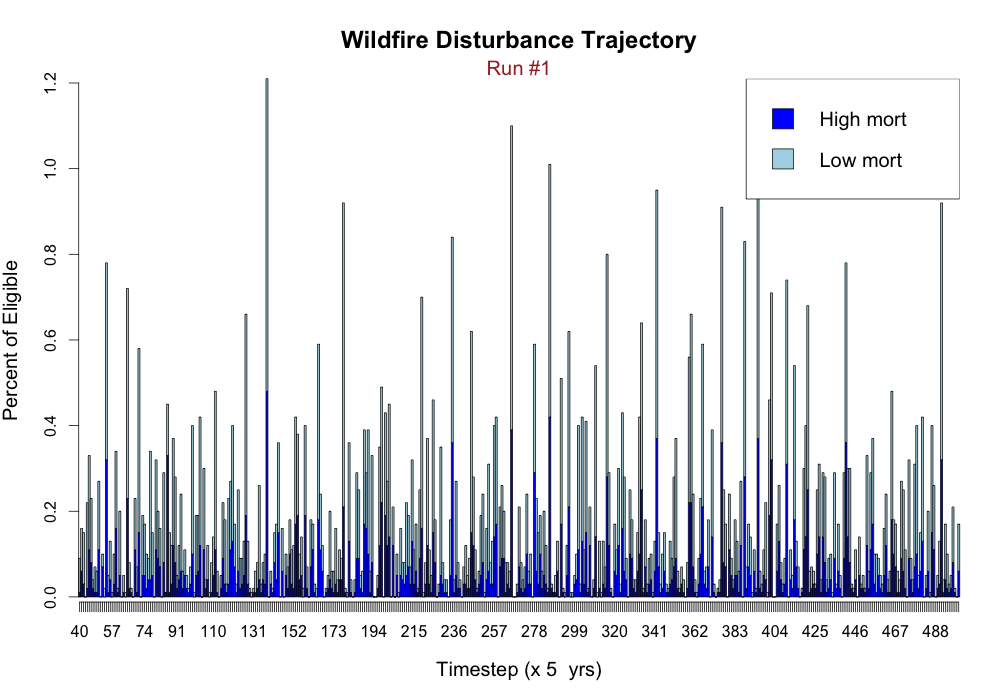
\includegraphics[width=0.5\textwidth]{/Users/mmallek/Tahoe/Report2/images/darea_smcu.png}
    }%
  \subfloat[][]{
    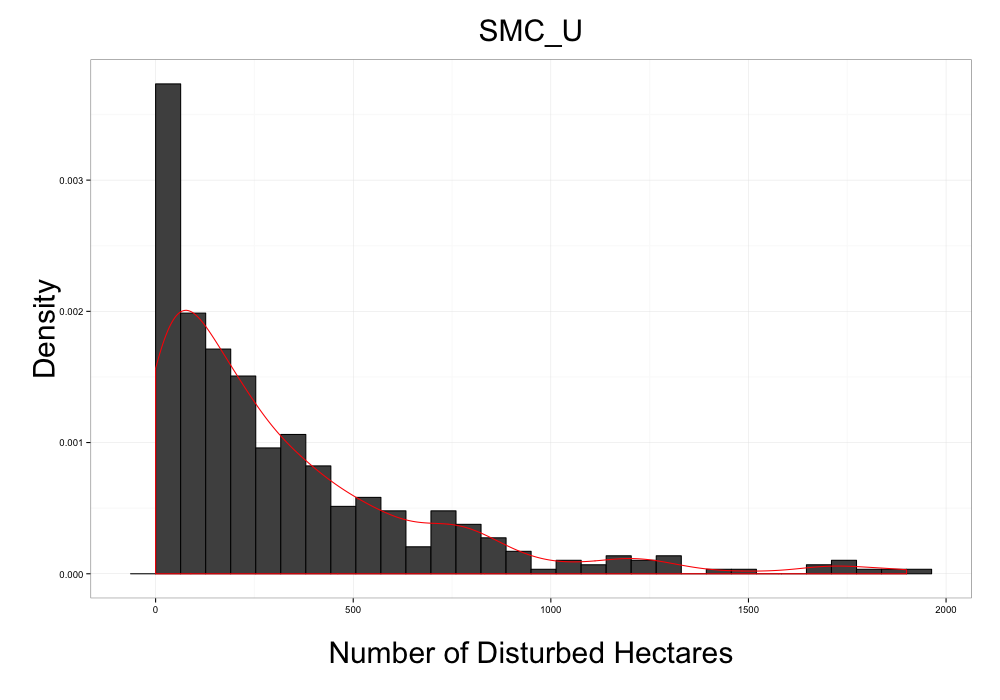
\includegraphics[width=0.5\textwidth]{/Users/mmallek/Tahoe/Report2/images/darea_hist_smcu.png}
    }
  \caption{\small (a) Disturbance trajectory for Sierran Mixed Conifer - Ultramafic. High mortality fire in dark blue; low mortality fire in light blue. (b) Histogram of disturbed hectares with density curve overlaid.} 
  \label{fig:darea_smcu}
\end{figure}

Sierran Mixed Conifer - Ultramafic (\textsc{smc\_u})is a relatively uncommon cover type within the core project area, encompassing 4,124 ha and comprising roughly 2\% of the project area. The frequency and extent of simulated wildfires in ultramafic sierran mixed conifer forests varied markedly across the landscape (Figure~\ref{fig:darea_smcu} and Table~\ref{tab:darea_smcu}).  %
%
Wildfire is much less common in this cover type compared to non-ultramafic sierran mixed conifer forests. Ultramafic soils support scattered, but rarely dense stands of trees and shrubs, creating fuel discontinuities that stop fires from spreading easily. Despite this, at least some area in ultramafic mixed conifer forest burned during all but one timestep. The burned extent was typically quite small: the median value for any fire was just 4\%, and less than 1\% of these forests (41 ha) burned during about 20\% of the simulated timesteps. The rarity of high mortality fire contributed to these statistics, which ordinarily burned just 1\% of the landscape. In general, however, fire was reasonably common, and over 10\% of the landscape burned about once every 19 years, which is much less common than for the other mixed conifer variants, as well as the oak-conifer ultramafic type. Even less likely were more widespread fires. Over 25\% of these forests burned on a 92 year interval, while over 50\% of the cover type only burned once during the simulation. The maximum extent burned within the cover type was about 50\% (about 2,100 ha). Still, low mortality fire was only about twice as common as high mortality fire, in contrast to the much larger differential found for ultramafic oak-conifer forests and woodlands. %
%
Under this wildfire regime, the grand mean return interval between fires (of any mortality level) varied widely from 20 years to over 500 years, with a median of 74 years (Figure~\ref{fig:preturn_smcu}). As expected, median return interval and rotation values are much longer for this cover type as compared to non-ultramafic mixed conifer forests, which occupy similar elevations. Ultramafic mixed conifer forests had a low mortality fire rotation of 106 years and a high mortality fire rotation of 196 years (Table~\ref{tab:darea_smcu}).  %
%
In general, return intervals and canopy cover varied spatially across the forest and decreased with increasing TPI, reflecting our parameterization, which was based on the theory that higher, more southerly aspects are drier and more susceptible to fires. Canopy cover decreased by about 36\% when comparing minimum to maximum TPI, from an average of 39\% to an average of 25\% (Table~\ref{tab:tpi_cc}). 


%%%
The age structure and dynamics of ultramafic mixed conifer forests illustrates the interaction between disturbance and succession processes. We focus our analysis on the 5$^{\text{th}}$ to 95$^{\text{th}}$ percentile range of variability for our simulation (excluding the equilibration period). %
%
The distribution of area among stand conditions within ultramafic mixed conifer forests fluctuated over time, as expected (Figure~\ref{fig:covcond_smcu}). For example, the percentage of ultramafic mixed conifer forests in the Mid Development - Open condition varied from 19\% to 30\%, reflecting the dynamic nature of this cover type (Table~\ref{tab:covcond2}). In both the current landscape and the simulation, patches in the Mid Development stage tended towards more open canopies, while patches in the Late Development stage tended towards more closed canopies. Ultramafic soils present a challenge to vegetation, which may explain the dominance of open conditions at the Mid Development stage. However, because fire is relatively uncommon, the shift in dominance at the Late Development stage may reflect the additional time available to vegetation to grow into a closed canopy condition (Appendix~\ref{sec:covertypedesc}). %
%
The seral-stage distribution appeared to be in dynamic equilibrium (i.e., the percentage in each stand condition varied about a stable mean). Our calculated current seral-stage distribution was never observed under the simulated HRV (Table~\ref{tab:covcond2}). The most notable departures were the decrease in area classified as Early Development---currently at 49\% of the landscape, but ranging from 27\%--41\% during the HRV---and the increase in area classified as Mid Development - Open---currently at 24\%, but ranging from 19\%--30\% during the HRV. Both Mid and Late Development - Closed are much more extensive on the current landscape than during the HRV, while Late Development - Open is much less extensive. The only cover type within the HRV was Mid Development - Moderate, which is in the $64^{\text{th}}$ percentile.

The spatial configuration of stand conditions fluctuated markedly over time as well, although there was considerable variation in the magnitude of variability among configuration metrics (Appendix \ref{sec:full-class-results}). Area-weighted patch and core area, as well as radius of gyration, exhibited the greatest variability over time. The class-level metrics for mesic mixed conifer forests do not consistently diverge from the HRV in one direction, nor are all classes outside the simulated HRV for our focal metrics. Patches in Early Development, Mid Development - Open, and Late Development - Closed were consistently outside the HRV for our focal metrics. Specifically, the first two types currently have fewer, larger patches that are more aggregated and contain more core area than during the HRV, while the opposite holds for Late Development - Closed. Results for the other condition classes generally fell within the HRV.

\begin{table}[!htbp]
\centering
\caption{\small Disturbed area summary statistics for Sierran Mixed Conifer - Ultramafic. Proportions shown are relative to the total area of Sierran Mixed Conifer - Ultramafic.}
\label{tab:darea_smcu}
\begin{tabular}{@{}llll@{}}
\toprule
\textbf{\begin{tabular}[c]{@{}l@{}}Summary Statistic \\ (disturbed area/timestep)\end{tabular}} & \textbf{Low Mortality} & \textbf{High Mortality} & \textbf{Any Mortality} \\ \midrule
Minimum       & 0.00	& 0.00 		& 0.00     \\
Maximum       & 30.77	& 20.25 	& 51.02        \\
Median        & 2.71	& 1.37 		& 4.25     \\
Mean          & 4.71	& 2.55 		& 7.27      \\
\textbf{Fire Rotation} & 106	& 196	& 69 \\  \bottomrule
\end{tabular}
\end{table}


%%%%%%%%%%%%%%%%%%%%%%%%%%%%%%%%%%%%%%%%%%%%%%%%%%%%%%%%%%%%%%%%%%%%%%%%%%%%%
%%%%%%%%%%%%%%%%%%%%%%%%%%%%%%%%%%%%%%%%%%%%%%%%%%%%%%%%%%%%%%%%%%%%%%%%%%%%%
%%%%%%%%%%%%%%%%%%%%%%%%%%%%%%%%%%%%%%%%%%%%%%%%%%%%%%%%%%%%%%%%%%%%%%%%%%%%%
%%%%%%%%%%%%%%%%%%%%%%%%%%%%%%%%%%%%%%%%%%%%%%%%%%%%%%%%%%%%%%%%%%%%%%%%%%%%%
%%%%%%%%%%%%%%%%%%%%%%%%%%%%%%%%%%%%%%%%%%%%%%%%%%%%%%%%%%%%%%%%%%%%%%%%%%%%%
%\clearpage
\section{Sierran Mixed Conifer - Xeric} 

\begin{figure}[!htbp]
  \centering
  \subfloat[][]{
    \centering
    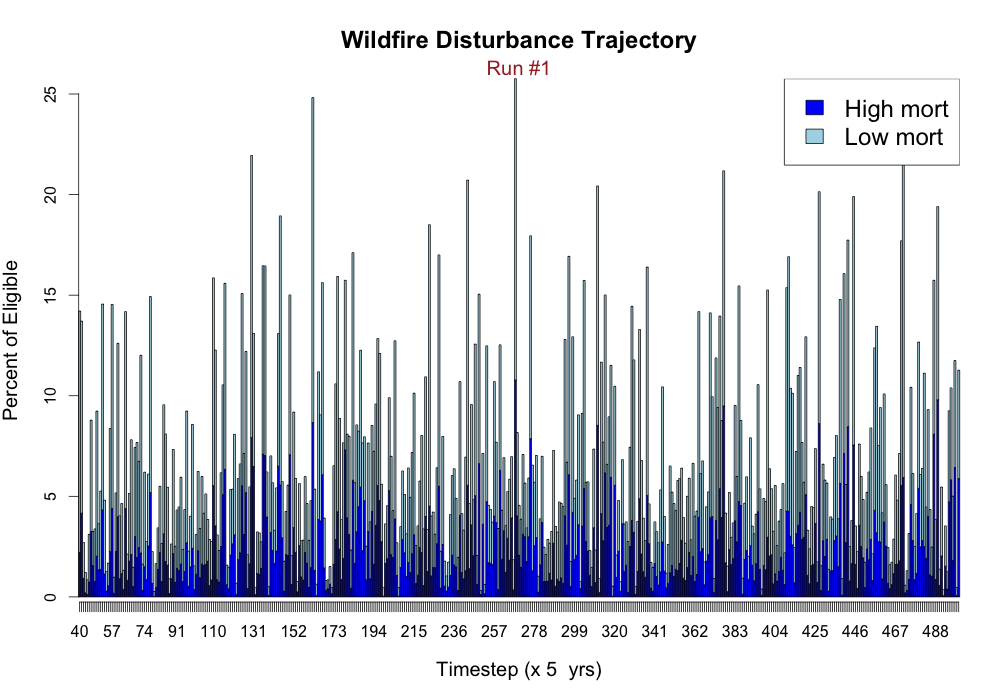
\includegraphics[width=0.5\textwidth]{/Users/mmallek/Tahoe/Report2/images/darea_smcx.png}
    }%
  \subfloat[][]{
    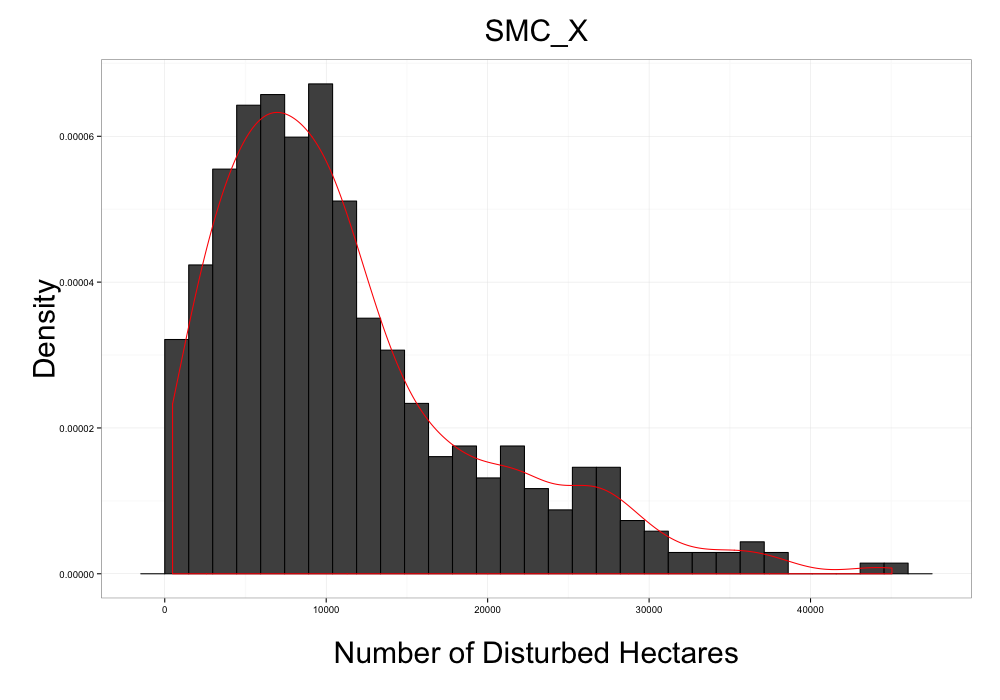
\includegraphics[width=0.5\textwidth]{/Users/mmallek/Tahoe/Report2/images/darea_hist_smcx.png}
    }
  \caption{\small (a) Disturbance trajectory for Sierran Mixed Conifer - Xeric. High mortality fire in dark blue; low mortality fire in light blue. (b) Histogram of disturbed hectares with density curve overlaid.} 
  \label{fig:darea_smcx}
\end{figure}

Sierran Mixed Conifer - Xeric (\textsc{smc\_x}) is the second most dominant cover type within the core project area, encompassing 52,198 ha and comprising roughly 29\% of the project area. The frequency and extent of simulated wildfires in xeric sierran mixed conifer forests varied markedly across the landscape (Figure~\ref{fig:darea_smcx} and Table~\ref{tab:darea_smcx}).  %
%
Wildfire is quite prevalent in xeric mixed conifer forests; its overall fire rotation is the lowest of all cover types. At least some area burned during every five-year timestep, and at least 10\% of the cover type burned in nearly 75\% of the simulated timesteps, or about every 7 years. The median amount of land burned during the simulation was 16\%. Over 25\% of the cover type burned every 18 years. Fires burned over 50\% of the cover type about once every 82 years, second only to oak-conifer forests and woodlands. During one five-year interval, 82\% of the xeric mixed conifer forest burned (around 42,700 ha). The minimum area burned was 186 hectares, which indicates a remarkable range of variability in disturbance extent. Low mortality fire was about 1.5 times as common as high mortality fire; both were a frequent occurence. %
%
Under this wildfire regime, the grand mean return interval between fires (of any mortality level) varied widely from 18 years to over 500 years, with a median of 24 years (Figure~\ref{fig:preturn_smcx}). As expected, median return interval and rotation values are much longer for this cover type as compared to non-ultramafic mixed conifer forests, which occupy similar elevations. Xeric mixed conifer forests had a low mortality fire rotation of 40 years and a high mortality fire rotation of 62 years (Table~\ref{tab:darea_smcx}), which was by far the lowest high mortality rotation period of any cover type. Neither high nor low mortality dominantes the disturbance regime. %
%
In general, return intervals and canopy cover varied spatially across the forest and decreased with increasing TPI, reflecting our parameterization, which was based on the theory that higher, more southerly aspects are drier and more susceptible to fires. Canopy cover decreased by about 21\% when comparing minimum to maximum TPI, from an average of 31\% to an average of 24\% (Table~\ref{tab:tpi_cc}).  %
%
Finally, when stands of xeric mixed conifer forests were adjacent to cover types with much shorter or longer return intervals, they also exhibited a directional shift in local return intervals towards that of the adjacent type, reflecting the importance of landscape context on fire regimes.


%%%
The age structure and dynamics of xeric mixed conifer forests illustrates the interaction between disturbance and succession processes. We focus our analysis on the 5$^{\text{th}}$ to 95$^{\text{th}}$ percentile range of variability for our simulation (excluding the equilibration period). %
%
The distribution of area among stand conditions within xeric mixed conifer forests fluctuated over time, as expected (Figure~\ref{fig:covcond_smcx}). For example, the percentage of xeric mixed conifer forests in the Early Development varied from 29\% to 49\%, reflecting the dynamic nature of this cover type (Table~\ref{tab:covcond3}). During the simulation, Early Development (which includes post-fire chaparral fields) and Mid Development - Open conditions dominated, in contrast to the current distribution, which is somewhat even across classes.  %
%
The seral-stage distribution appeared to be in dynamic equilibrium (i.e., the percentage in each stand condition varied about a stable mean). Our calculated current seral-stage distribution was never observed under the simulated HRV (Table~\ref{tab:covcond3}). In fact, none of the condition classes had a distribution within the simulated HRV. The most notable departure was the increase in Early Development and Mid Development - Open during the simulated HRV compared to the current landscape (currently at 19\% and 11\%, respectively). We also observed a much lower proportion of xeric mixed conifer forest in Late Development - Closed during the simulation than in the current landscape (25\%). The decline in the extent of Late Development forests is primarily due to the frequency of high mortality fire, which inhibits stands from succeeding to those stages. High mortality fire directly led to the increase in Early Development conditions, and the dominance of open canopies within the Mid Development stage is explained by the high frequency of low mortality fire.

The spatial configuration of stand conditions fluctuated markedly over time as well, although there was considerable variation in the magnitude of variability among configuration metrics (Appendix \ref{sec:full-class-results}). Area-weighted patch and core area, as well as edge density, exhibited the greatest variability over time. The magnitude of the shift from the median values during the simulated HRV is consistently high across class metrics, with many falling completely outside the HRV. However, the direction of that shift is not always consistent, breaking the cover type into two groups: Early Development and Mid and Late Development - Open in one, and the remaining condition classes in the other. During the HRV, most of the landscape was comprised of cover types in the first group. Patches classified into these conditions are currently smaller in area and core area, and less numerous, aggregated, and geometrically complex than during the simulated HRV.


\begin{table}[!htbp]
\centering
\caption{\small Disturbed area summary statistics for Sierran Mixed Conifer - Xeric. Proportions shown are relative to the total area of Sierran Mixed Conifer - Xeric.}
\label{tab:darea_smcx}
\begin{tabular}{@{}llll@{}}
\toprule
\textbf{\begin{tabular}[c]{@{}l@{}}Summary Statistic \\ (disturbed area/timestep)\end{tabular}} & \textbf{Low Mortality} & \textbf{High Mortality} & \textbf{Any Mortality} \\ \midrule
Minimum       & 0.27	& 0.04	  & 0.36   \\
Maximum       & 50.08	& 34.21	  & 81.77       \\
Median        & 9.62	& 6.04	  & 16.17    \\
Mean          & 12.35	& 8.11	  & 20.46     \\
\textbf{Fire Rotation} & 40	& 62	& 24 \\  \bottomrule
\end{tabular}
\end{table}





